\section{S-matrix elements}
\emph{Note: I was unable to make it to this lecture due to travel constraints, so these notes are adapted from Inci's lecture notes - many thanks!}

\subsection{Review of the LSZ Formula}
Before the break, we discussed the LSZ formula, which allowed us to convert observables (specifically, time-ordered correlators) into S-matrices (i.e. scattering/transition amplitudes).

In more detail, recall that the $S$-matrix consists of amplitudes $\braket{f}{i}$ for a specific in state, e.g. $\ket{i} = a^\dag_{\v{k}_1}(-\infty)a^\dag_{\v{k}_2}(-\infty)\ket{0}$ to evolve into a specific out state, e.g. $\bra{f} = \bra{0}a_{\v{k}_1'}(\infty)a_{\v{k}_2'}(\infty)$. The LSZ formula relates this matrix element to a time-ordered correlator:
\begin{equation}
    \braket{f}{i} = i^4\int_{x_1, x_2, x_1', x_2'}e^{i(k_1x_1 + k_2x_2 - k_1'x_1' - k_2'x_2')}(m^2 - \p_1^2)(m^2 - \p_2^2)(m^2 - \p_{1'}^2)(m^2 - \p_{2'}^2)\bra{0}\mathcal{T}\set{\phi(x_1)\phi(x_2)\phi(x_1')\phi(x_2')}\ket{0}
\end{equation}
Note that the $k_i$ appearing in the above are 4-momenta, with the $k_i^0$/energy being fixed by the spatial momentum:
\begin{equation}
    k_i^0 = \e_{\v{k}_i} = \sqrt{m^2 + \v{k}_i^2}
\end{equation}
The S-matrix is thus an ``on-shell'' observable.

We also note that in order for the normalization to be correct (in interacting theories $\bra{\v{k}}a_{\v{k}'}^\dag(-\infty)\ket{0} = C\delta(\v{k} - \v{k'})$ with $C$ not necessarily 1), we normalize the fields such that $\bra{\v{k}}\phi(0)\ket{0} = 0$, so:
\begin{equation}
    \bra{\v{k}}\phi(x)\ket{0} = e^{ikx}\bra{k}\phi(0)\ket{0} = e^{ikx}
\end{equation}

\subsection{S-matrix for interacting scalar QFT}
We consider the Lagrangian:
\begin{equation}
    \mathcal{L} = -\frac{1}{2}(\p\phi)^2 - \frac{1}{2}m^2\phi^2 - \frac{1}{3!}g\phi^3 - \frac{1}{4!}\lambda\phi^4
\end{equation}
Integrating the LSZ formula by parts twice, we obtain the expression:

\begin{equation}
    \bra{f}{i} = (m^2 + k_1^2)(m^2 + k_2^2)(m^2 + k_1'^2)(m^2 + k_2'^2)\int_{x_1, x_2, x_1', x_2'}e^{ik_1x_1 + k_2x_2 - k_1x_1' - k_2x_2'}\avg{\phi(x_1)\phi(x_2)\phi(x_1')\phi(x_2')}
\end{equation}
where we have the time ordered correlator:
\begin{equation}
    \begin{split}
        \avg{\phi(x_1)\phi(x_2)\phi(x_1')\phi(x_2')} &\equiv \avg{\phi(x_1)\phi(x_2)\phi(x_1')\phi(x_2')}_C 
        + \avg{\phi(x_1)\phi(x_1')}\avg{\phi(x_2)\phi(x_2')} 
        \\ &+ \avg{\phi(x_1)\phi(x_2')}\avg{\phi(x_2)\phi(x_1')} + \avg{\phi(x_1)\phi(x_2)}\avg{\phi(x_1')\phi(x_2')} 
    \end{split}
\end{equation}
Note that since $k_1, k_2, k_1', k_2'$ make up our ``on-shell'' 4-point function, it seems like the $m^2 + k_i^2$ gives zero, but the connected part will always have $G(k_1)G(k_2)G(k_1')G(k_2')$ which cancels out the zeroes.

\subsection{Disconnected Terms and the Free-Field S-Matrix}
We look at the disconnected terms in the above matrix element. The first is:
\begin{equation}
    (1) = \int_{x_1, x_2, x_1' x_2'}e^{i(k_1x_1 + k_2x_2 - k_1'x_1' - k_2'x_2')}G(x_1' - x_1) G_2(x_2' - x_2)
\end{equation}
with $G(x) = G_F(x) = \bra{0}\mathcal{T}\set{\phi(x)\phi(0)}\ket{0}$. Defining $\tilde{x}_i = x_i' - x_i$ we have:
\begin{equation}
    (1) = \int_{x_1, x_2, x_1', x_2'}e^{ix_1(k_1 - k_1')}e^{ix_2(k_2 - k_2')}e^{-ik_1'\tilde{x}_1}G(\tilde{x}_1)e^{-ik_2'\tilde{x}_2}G(\tilde{x}_2) = G(k_1')G(k_2')(2\pi)^{d+1}\delta^{d+1}(k_1-k_1')(2\pi)^{d+1}\delta^{d+1}(k_2 - k_2'
    )
\end{equation}
where in the second equality we Fourier transform the $e^{-ik_i'\tilde{x}_i}G(\tilde{x}_i)$s. Thus we have the nonzero term represented by the diagram:

\begin{center}
    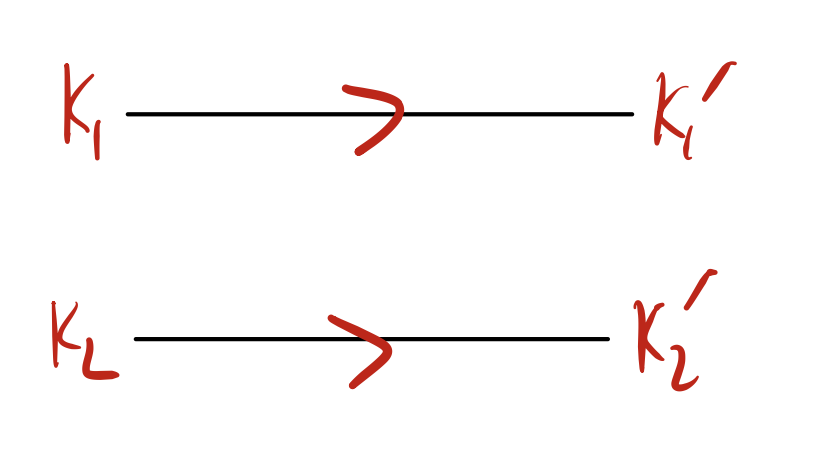
\includegraphics[scale=0.35]{Lectures/Figures/lec17-stay.png}
\end{center}

For the second disconnected term, we can follow the same procedure and obtain:
\begin{equation}
    (2) = G(k_1)G(k_2)(2\pi)^{d+1}\delta^{d+1}(k_1 - k_2')(2\pi)^{D+1}\delta^{d+1}(k_2 - k_1')
\end{equation}
which is represented by the diagram:

\begin{center}
    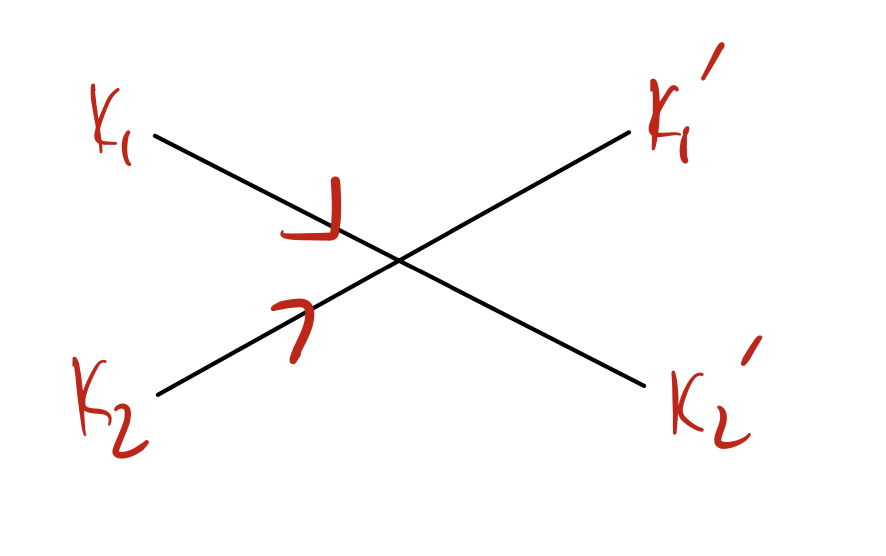
\includegraphics[scale=0.35]{Lectures/Figures/lec17-swap.png}
\end{center}

Technically, there is also a third term with $\delta^{d+1}(k_1 + k_2)$. But, this term is associated with two physical momenta/particles, i.e. $k_1^0, k_2^0 > 0$ and hence vanishes, with $\delta^{d+1}(k_1 + k_2) = 0$.

In the free theory, this would be it! We would have:
\begin{equation}
    \bra{0}a_{k_1'}a_{k_2'}a^\dag_{k_1}a^\dag_{k_2}\ket{0} = 2\e_{k_1}\e_{k_2}(2\pi)^{2(d+1)}\left[\delta^d(\v{k}_1 - \v{k}_1')\delta^d(\v{k}_2 - \v{k}_2') + \delta^d(\v{k}_1 - \v{k}_2')\delta^d(\v{k}_2 - \v{k}_1')\right]
\end{equation}
and thus obtain $\braket{f}{i} = \delta_{if}$, i.e. the $S$ matrix is the identity:
\begin{equation}
    S = 1
\end{equation}
This makes physical sense; in the free theory there is no interaction/scattering process between the particles, so all that can happen is the initial state stays the same to the final state.

\subsection{First-Order connected Term}
In an arbitrary interacting theory, we isolate the non-trivial scattering part of the $S$-matrix by writing:
\begin{equation}
    \braket{f}{i} = \delta_{if} + T_{if}
\end{equation}
or $S = 1 + iT$. The $T$ represents the non-trivial part. For the interacting scalar QFT we have written, this term looks like:
\begin{equation}
    T_{if} = (m^2 + k_1^2)(m^2 + k_2^2)(m^2 + k_1'^2)(m^2 + k_2'^2)\int_{x_1, x_2, x_1', x_2'}e^{ik_1x_1 + k_2x_2 - k_1x_1' - k_2x_2'}\avg{\phi(x_1)\phi(x_2)\phi(x_1')\phi(x_2')}_C
\end{equation}
where we have subtracted off the free field theory contribution.

Let us evaluate this. We use translation invariance of the theory to simplify our life, substituting $x_1 \to x_1 + x_2'$, $x_2 \to x_2 + x_2'$, $x_1' \to x_1' + x_2'$. We then have:
\begin{equation}
    \avg{\phi(x_1)\phi(x_2)\phi(x_1')\phi(x_2')}_C = \avg{\phi(x_1 - x_2')\phi(x_2-x_2')\phi(x_1-x_2')\phi(0)}_C \equiv \avg{\phi(x_1)\phi(x_2)\phi(x_1')\phi(0)}_C 
\end{equation}
where in the last equality we use our new renamed variables.
Thus:
\begin{equation}
    T_{if} = (m^2 + k_1^2)(m^2 + k_2^2)(m^2 + k_1'^2)(m^2 + k_2'^2)\int_{x_1, x_2, x_1', x_2'}e^{ik_1x_1 + k_2x_2 - k_1x_1' - k_2x_2'}\avg{\phi(x_1)\phi(x_2)\phi(x_1')\phi(0)}_C = (2\pi)^{d+1}\delta^{d+1}(k_1 + k_2 - k_1' - k_2')i\mathcal{M}.
\end{equation}
Where in the last equality we Fourier transform and define  $\mathcal{M}$ as the matrix element, with:
\begin{equation}
    i\mathcal{M} = (m^2 + k_1^2)(m^2 + k_2^2)(m^2 + k_1'^2)(m^2 + k_2'^2)\avg{\phi_{k_1}\phi_{k_2}\phi_{-k_1'}\phi(0)}_C
\end{equation}
with $\phi_{k_i} = \int_{x_i}e^{i x_ik_i}\phi(x_i)$. As usual. For the free theory,$\avg{\phi_{k_1}\phi_{k_2}\phi_{-k_1'}\phi(0)}_C = 0$ and $\mathcal{M}$ vanishes.

Let us compute the matrix element to leading order in the coupling; there is no $O(g)$ contribution at this order, but we will find a $O(\lambda)$ contribution:
\begin{equation}
    \avg{\phi_{k_1}\phi_{k_2}\phi_{-k_1'}\phi(0)}_C \sim \avg{\phi_{k_1}\phi_{k_2}\phi_{-k_1'}\phi(0)\left(\frac{-i}{4!}\lambda \int_x \phi^4(x)\right)}_{g,\lambda = 0}
\end{equation}
There are $4 \cdot 3 \cdot 2 \cdot 1 = 4!$ ways of ordering the fields/choices for Wick contractions, which cancels out with the $\frac{1}{4!}$ present in the interaction term of the Lagrangian.

Looking at the types of contractions, we have:
\begin{equation}
    \wick{\c1 \phi(x) \c1 \phi(0)} = G(x)
\end{equation}
\begin{equation}
    \wick{\c1 \phi(x) \c1 \phi_k} = \int_{x'}e^{ikx'}\wick{\c1 \phi(x) \c1 \phi(x')} = \int_{x'}G(x' - x) \stackrel{\tilde{x} = x' - x}{=} e^{ikx}\int_{\tilde{x}} e^{ik\tilde{x}}G(\tilde{x}) = e^{ikx}G(k)
\end{equation}
Thus:
\begin{equation}
    \begin{split}
        \avg{\phi_{k_1}\phi_{k_2}\phi_{-k_1'}\phi(0)}_C = -i\lambda\int_{x}e^{i(k_1 + k_2 - k_1')x}G(k_1)G(k_2)G(k_1')G(x) &= -i\lambda G(k_1)G(k_2)G(k_1')G(k_1 + k_2 - k_1') 
        \\ &= -i\lambda G(k_1)G(k_2)G(k_1')G(-k_2')
    \end{split}
\end{equation}
Graphically, we have the diagram:

\begin{center}
    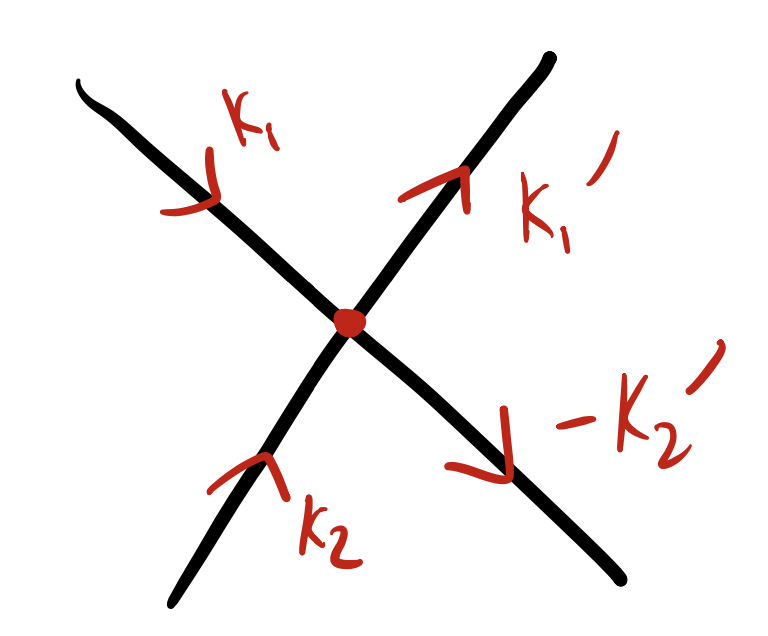
\includegraphics[scale=0.3]{Lectures/Figures/lec17-4pointvertex.png}
\end{center}

Note that all the $G(\cdot)$ cancel out the prefactors, since $G(k) = \frac{-i}{k^2 + m^2}$. Thus we find that $i\tilde{M}_{i \to f} = -i\lambda$, or that:
\begin{equation}
    \tilde{M}(\v{k}_1, \v{k}_2 \to \v{k}_1', \v{k}_2') = -\lambda
\end{equation}
Note that we have no $\v{k}$ dependence! this is the simplest $S$-matrix.

\subsection{Higher-Order S-Matrix}

If we look at $O(g^2)$, we then have $\phi^3$ terms, which result in a non-trivial $S$-matrix. Let's look at this:
\begin{equation}
    \avg{\phi_{k_1}\phi_{k_2}\phi_{-k_1'}\phi(0)}_C \cong \frac{(-i)^2}{2}\left(\frac{g}{3!}\right)^2\int_{x, y}\avg{\phi_{k_1}\phi_{k_2}\phi_{-k_1'}\phi(0)\phi^3(x)\phi^3(y)}
\end{equation}
As is now standard, we can now count all the possible Wick contractions. $\phi(0)$ can contract with either $\phi(x)$ or $\phi(y)$, of which there are 3 each, which gives $3 \cdot 2$ contractions. At least one of the $\phi(x)$ and $\phi(y)$ must contract with each other, else the diagram is disconnected - since there are 2 remaining $\phi(x)$s and 3 remaining $\phi(y)$s (or vise versa), there is another factor of $3 \cdot 2$ contractions. Together this cancells out the $\frac{1}{3!^2}$ factor on the outside. Of the remaining fields, the last $\phi(x)$ contracts with one of $\phi_{k_1}, \phi_{k_2}, \phi_{-k_1'}$ and the other two contract with the remaining $\phi(y)$s. We can classify the diagrams we get based on which of the external momenta the $\phi(x)$ gets contracted with:

\begin{itemize}
    \item If $\phi(x)$ contracts with $\phi_{k_1'}$, then we have the S-channel:
    \begin{equation}
        \equiv -g^2\int_{x, y}e^{i(k_1 + k_2)y}G(k_1)G(k_2)e^{-ik_1'x}G(k_1')G(x)G(x-y)
    \end{equation}
    \begin{center}
        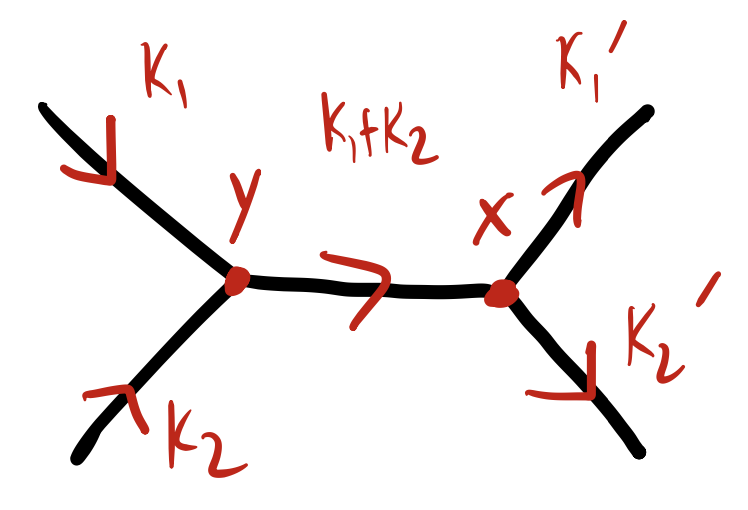
\includegraphics[scale=0.35]{Lectures/Figures/lec17-schannel.png}
    \end{center}

    \item If $\phi(x)$ contracts with $\phi_{k_1}$, then we have the u-channel:
    \begin{equation}
        \equiv -g^2\int_{x, y}e^{i(k_2 - k_1')y}e^{ik_1x}G(k_1)G(k_2)G(k_1')G(x)G(x-y)
    \end{equation}
    \begin{center}
        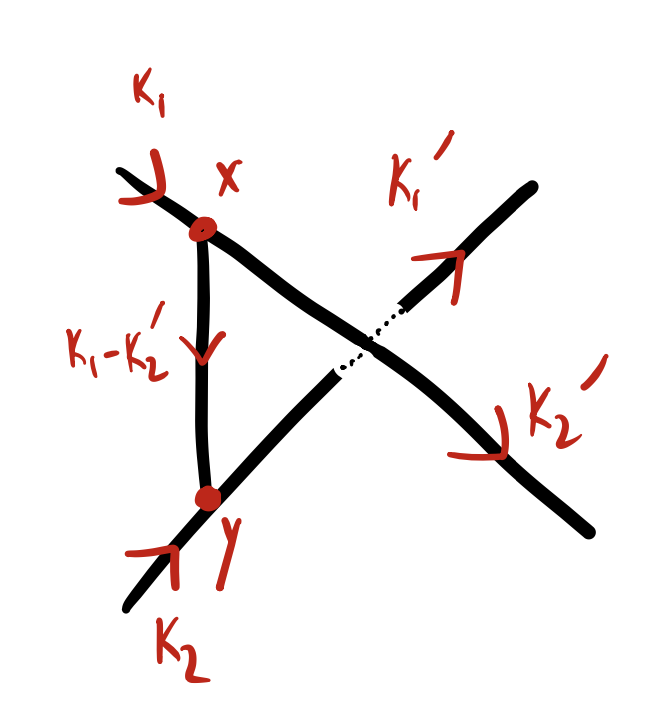
\includegraphics[scale=0.35]{Lectures/Figures/lec17-uchannel.png}
    \end{center}

    \item If $\phi(x)$ contracts with $\phi_{k_2}$, we have the t-channel:
    \begin{equation}
        \equiv -g^2\int_{x, y}e^{i(k_1 - k_1')y}G(k_1)e^{ik_2x}G(k_2)G(k_1')G(x)G(x-y)
    \end{equation}
    \begin{center}
        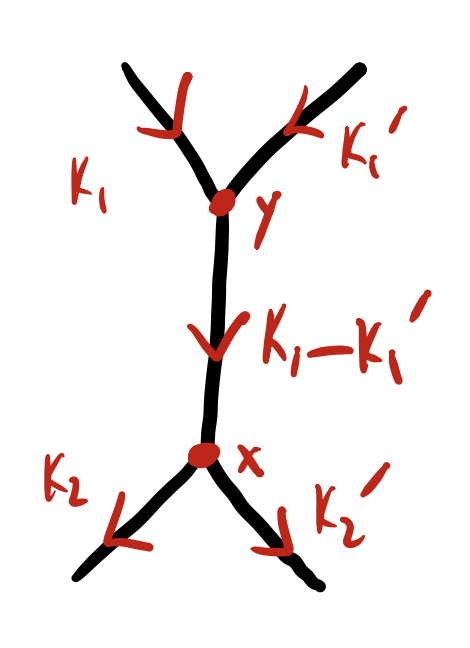
\includegraphics[scale=0.35]{Lectures/Figures/lec17-tchannel.png}
    \end{center}
\end{itemize}

Thus with $\tilde{y} = x - y'$, we have the matrix element:
\begin{equation}
    \begin{split}
        i\mathcal{M} &= i(m^2 + k(k_1 + k_2 - k_1')^2)(-g^2)\int_{x, \tilde{y}}e^{-ix(k_1 + k_1 - k_1')}G(x)\left[e^{-i(k_2 - k_1')\tilde{y}}G(\tilde{y}) + e^{-i(k_1 - k_1')}G(\tilde{y}) + e^{-i(k_1 + k_2)}G(\tilde{y})\right]
        \\ &= -g^2\left[G(k_1 - k_1') + G(k_1 - k_1') + G(k_1 + k_2)\right] 
        \\ &= ig^2\left[\frac{1}{m^2+ (k_2 - k_1')^2} + \frac{1}{m^2 + (k_1 - k_1')^2} + \frac{1}{m^2 + (k_1 + k_2)^2}\right]
    \end{split}
\end{equation}